\section{Theoretical models}\label{sec:model}
\subsection{Thermal statistical model}

The statistical-thermal model has proved extremely successful in applications to relativistic collisions of both heavy ions and elementary particles as shown in Figure \ref{fig:thermal}. In light of this success, THERMUS, a thermal model analysis package, has been developed for incorporation into the object-oriented ROOT framework \cite{Wheaton:2004qb}.\\ 

\begin{figure}[htbp]
\begin{center}
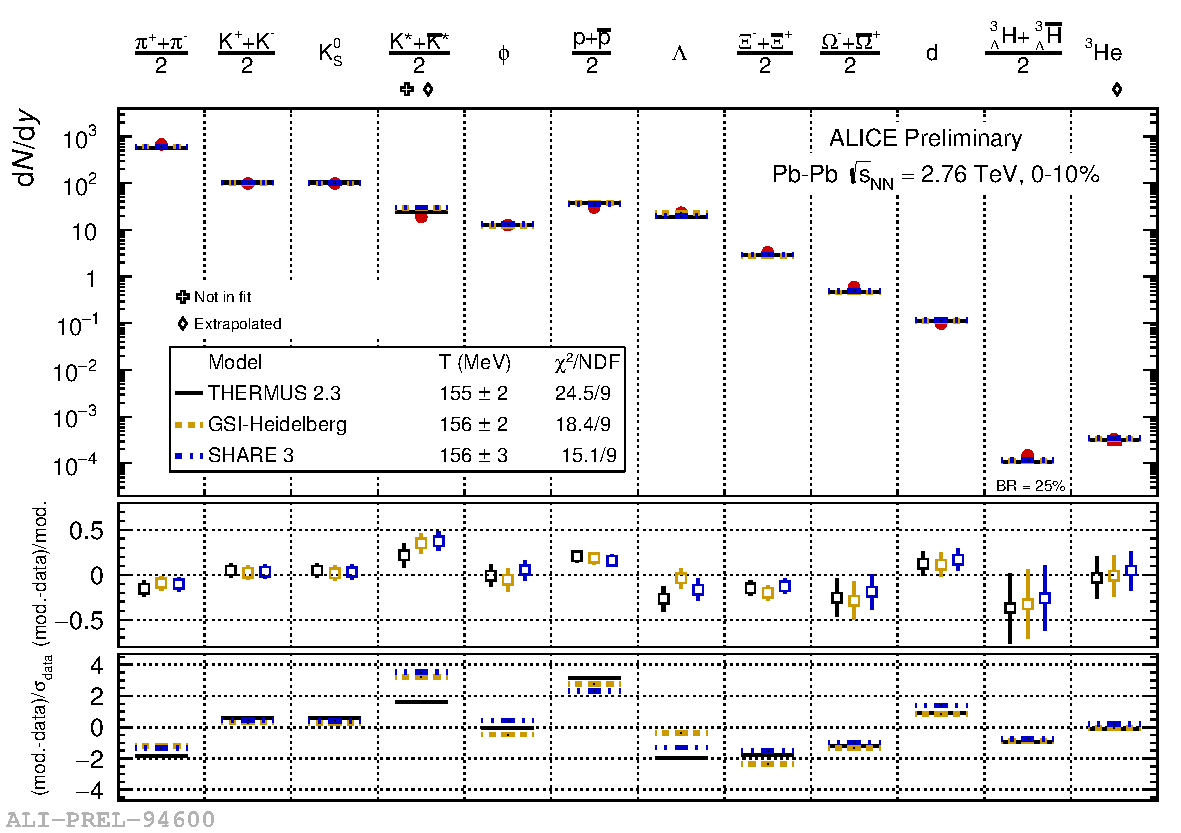
\includegraphics[width=14.cm]{./Version1/FigChapter2/ThermalModel}
\caption{Grand canonical thermal fit of 0-10\% central Pb-Pb collisions, with 3 models (THERMUS, GSI, SHARE). Excluded volume correction implemented in THERMUS and GSI with rh = 0.3 fm $\mu_{B}$ fixed to 0, $\gamma_{s}$ fixed to 1, $\gamma_{c}$ fixed to 20 (THERMUS and GSI)}
\label{fig:thermal}
\end{center}
\end{figure}


There are three types of statistical-thermal models in explaining data in high energy nuclear physics and THERMUS treats the system quantum numbers B (baryon number), S (strangeness) and Q (charge) within three distinct formalisms: 

\begin{enumerate}
\item \textbf{Grand-Canonical Ensemble:} Because the hot dense matter produced in nucleus-nucleus collisions is large enough, this ensemble is the most widely used in applications to heavy-ion collisions, in which the quantum numbers are conserved on average. 
\item \textbf{Fully-Canonical Ensemble:} In which B, S and Q are each exactly conserved and this ensemble used in high-energy elementary collisions such as pp, p\pbar{} and e$^{-}$e$^{+}$ collisions.
\item \textbf{Strangeness-Canonical Ensemble:}  In small systems or at low temperatures, a canonical treatment leads to a suppression of hadrons carrying non-zero quantum numbers, since these particles have to be created in pairs and the resulting low production of strange particles requires a canonical treatment of strangeness.  
 \end{enumerate}
 In order to calculate the thermal properties of a system, one starts with an evaluation of its partition function. The form of the partition function obviously depends on the choice of ensemble. In the present analysis the strangeness-canonical ensemble used and the statistical-thermal model requires six parameters as input: the chemical freeze-out temperature $T$, baryon and charge chemical potentials $\mu_{B}$ and $\mu_{Q}$ respectively, canonical or correlation radius, $R_{C}$; the radius inside which strangeness is exactly conserved and the fireball radius $R$. An additional strangeness saturation factor $\gamma_{S}$ has been used as indicator of a possible departure from equilibrium and $\gamma_{S}=1.0$ corresponds to complete strangeness equilibration.
 

The volume dependence cancels out when studying the particle ratios as well as strangeness canonical equivalent to grand canonical formalism if $\Delta S=0$ in the ratios and $\gamma_{S}$ also cancels out. Parameters used in the analysis listed in Table~\ref{jfonts}. The $\mu_{B}$ parameter taken from the Ref.~\cite{Cleymans:2011pe}.
 
 \begin{center}
\begin{table}[h]
\centering
\caption{\label{jfonts} Parameters used in the thermal-model calculations.} 
%\begin{tabular}{@{}l*{15}{l}}
 \begin{tabular}{@{}*{2}{cc}}
\hline
Parameter&Value\\
\hline
$T$ (MeV)&varied (see text)\\
$\mu_{B}$ (MeV)&$9.2\times10^{-2}$????\\ 
$\mu_{Q}$ (MeV)&$0.0$\\ 
$\gamma_{S}$&$1.0$\\ 
%$R_{C}$ (fm)&$1.5$\\ 
%$R$ (fm)&$4.0$\\ 
\hline
\end{tabular}
\end{table}
\end{center}
\newpage
\subsubsection{Calculations}
\textit{Concept:} \\In order to calculate the particle ratios within strangeness canonical formalism of THERMUS, temperature varied between 60 MeV to 180 MeV and particle yields extracted for each temperature value and then primary particle ratios calculated for each case. \\ \\
\textit{Feed-Down Correction:} \\Since the particle yields measured by the detectors in collision experiments include feed-down from heavier hadrons and hadronic resonances, the primordial hadrons are allowed to decay to particles considered stable by the experiment before model predictions are compared with experimental data. In the analysis only  $\Lambda$ particles counted as stable (do not allowed to decay) so there is no feed-down contribution from these particles to the other ratios.  \\ \\

Properties of studied particles and their particle ratios listed in Table~\ref{opt} and Table~\ref{diff}, respectively. 
%\begin{landscape}

%\begin{center}
%\begin{table}[h]
\hspace*{-1cm}
\begin{table}[!htb] 
\hspace*{-1cm}
%\vspace{1.5 cm}
\caption{\label{opt} Properties of particles used in the ratio calculations.}
%
\hspace*{-1cm}
%
%\addtolength{\tabcolsep}{-2.7pt}
 \begin{tabular}{lcccccccccccc}
\hline
\hline
Particle&$\Delta^{++}$ &  p & K$^{*0}$ &K$^{0} $ &K$^{+} $ & $\Lambda^{*}$ & $\Lambda$& $\Sigma^{*+}$  & $\Sigma^{+}$ & $\Sigma^{0}$ & $\Xi^{*0}$ & $\Xi^{-}$\\
\hline
Mass (MeV/$c^{2}$)&1232&938.27&895.92&497.61&493.67&1519.5&1115.68&1382.8&1189.37&1192.64&1531.80&1321.31\\
%\hline 
Width (MeV/$c^{2}$)&120&--&50.7&--&--&15.6&--&37.6&--&--&9.1&--\\
%\hline
$c\tau$ (fm)&1.6&--&3.9&--&--&12.6&--&5.51&--&--&$21.6$&--\\
%\hline
Ang. Momentum ($J$)&3/2&1/2&1&1&0&3/2&1/2&3/2&1/2&1/2&3/2&1/2\\
%\hline
Isospin ($I$)&3/2&1/2&1/2&1/2&1/2&0&0&1&1&1&1/2&1/2\\
%\hline
Parity ($P$)&+1&+1&-1&-1&0&-1&+1&+1&+1&+1&+1&+1\\
%\hline
Strangeness ($S$)&0&0&1&1&1&-1&-1&-1&-1&-1&-2&-2\\
%\hline
Baryon Number ($B$)&1&1&0&0&0&1&1&1&1&1&1&1\\
%\hline
Decay Channel&p$\pi^{+}$&--&$\pi^{-}$&--&$\mu^{+}\nu_{\mu}$&pK$^{-}$&$p\pi^{-}$&$\Lambda\pi^{+}$&p$\pi^{0}$&$\Lambda\gamma$&$\Xi^{-}\pi^{+}$&$\Lambda\pi^{-}$\\
%\hline
Branching Ratio (\%)&$\sim100$&--&$\sim66.7$&--&$\sim63.54$&$\sim45$&$\sim63.9$&$\sim87$&$\sim51.6$&$\sim100$&$\sim64$&$\sim99.9$\\
Q-Value(MeV/$c^{2}$)&154.16&--&262.68&--&--&87.55&37.84&127.55&111.53&76.96&70.92&70.66\\
 \hline
 \hline
\end{tabular}
\end{table}
%\end{center}

\vspace{6pt}
 \begin{center}
\begin{table}[!htb] 
\caption{\label{diff} Difference of mass ($\Delta M$), baryon number ($\Delta B$), strangeness ($\Delta S$) and charge ($\Delta Q$) of the ratios. The values of the slopes needs to be checked!!!!}
\centering
 \begin{tabular}{lcccccccc}
 	 		\hline
\hline
Particle&$\Delta^{++}$/p & K$^{*}$/K$^{+}$& $\Lambda^{*}/\Lambda$&$\Sigma^{*+}/\Lambda$  &$\Sigma^{*+}/\Sigma^{0}$ &$\Sigma^{0}/\Lambda$ & $\Sigma^{*+}/\Sigma^{+}$ & $\Xi^{*0}/\Xi^{-}$\\
\hline
\textit{$\Delta M$ ({\rm MeV}/$c^{2}$)}&293.8&402.25&403.82&267.12&190.16&76.96&193.43&210.49\\
\textit{$\Delta B$}&0&0&0&0&0&0&0&0\\
\textit{$\Delta S$}&0&0&0&0&0&0&0&0\\
\textit{$\Delta Q$}&+1&-1&0&+1&0&+1&0&-1\\
%\textit{Q-Value ($MeV/c^{2}$)}&154.16&262.68&87.55&87.55&127.55&127.55&76.96&127.55&70.92\\
\hline
Slope (\%) per MeV ??????& 0.19 &0.76& 0.98& 0.25 & - & -0.08 &0.37 &0.42\\
 \hline
\end{tabular}
\end{table}
\end{center}
%\end{landscape}

%\newpage	

\subsubsection{Results and comparison with data}
\begin{figure}[!htbp]
\begin{center}
        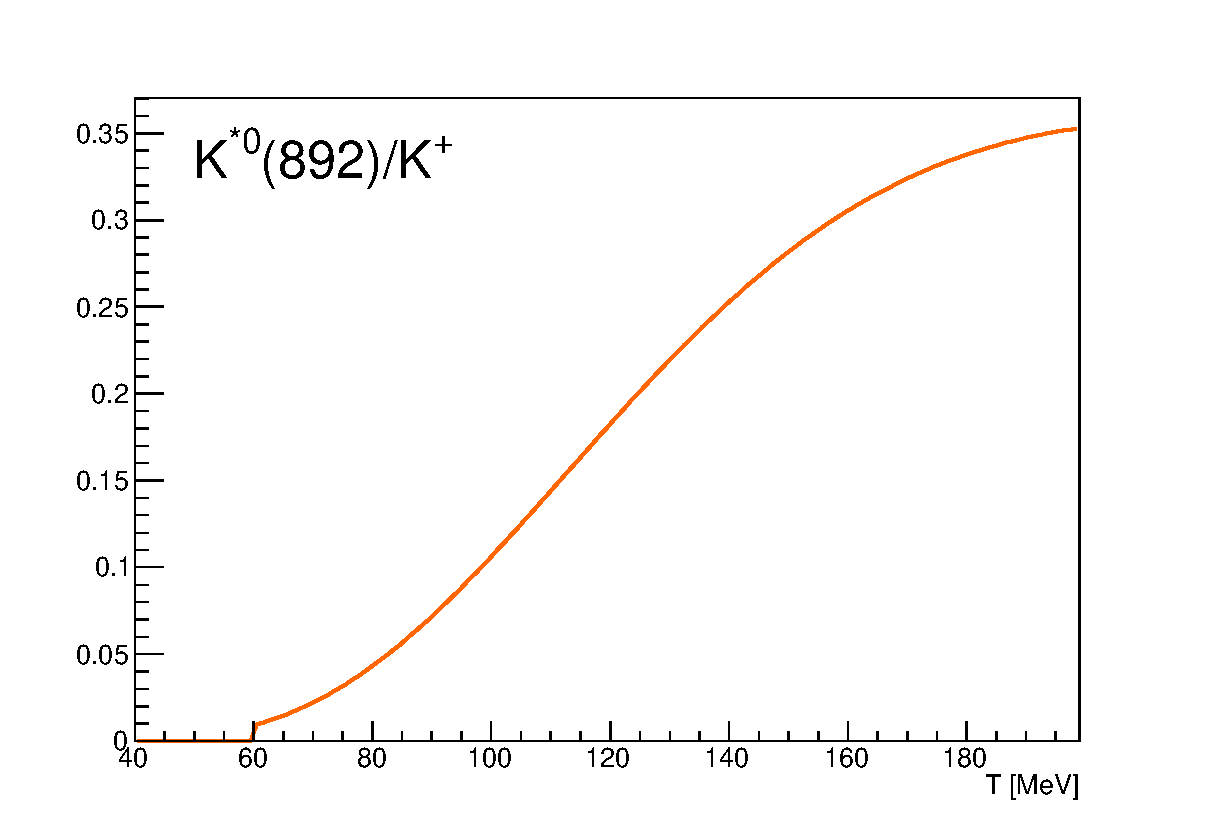
\includegraphics[width=200px]{./Version1/FigChapter2/KStarToK}
       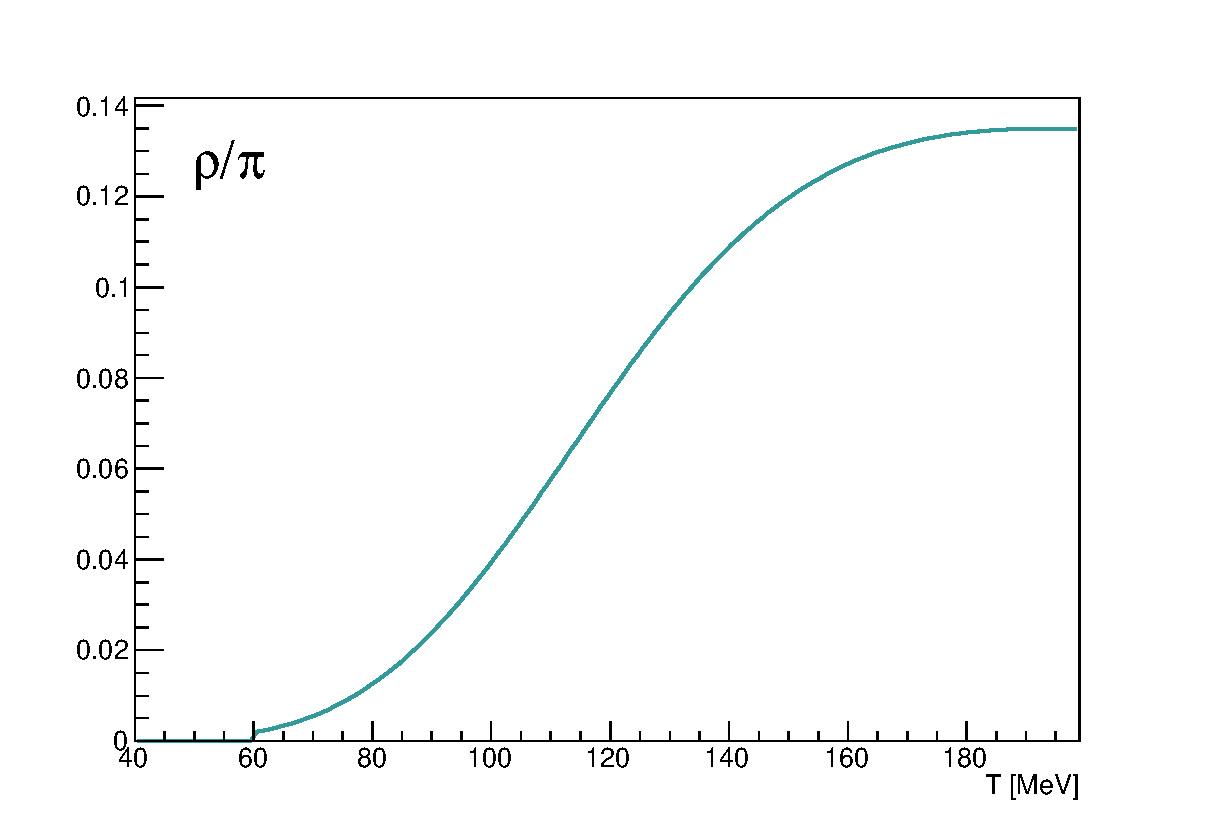
\includegraphics[width=200px]{./Version1/FigChapter2/RhoToPion}
        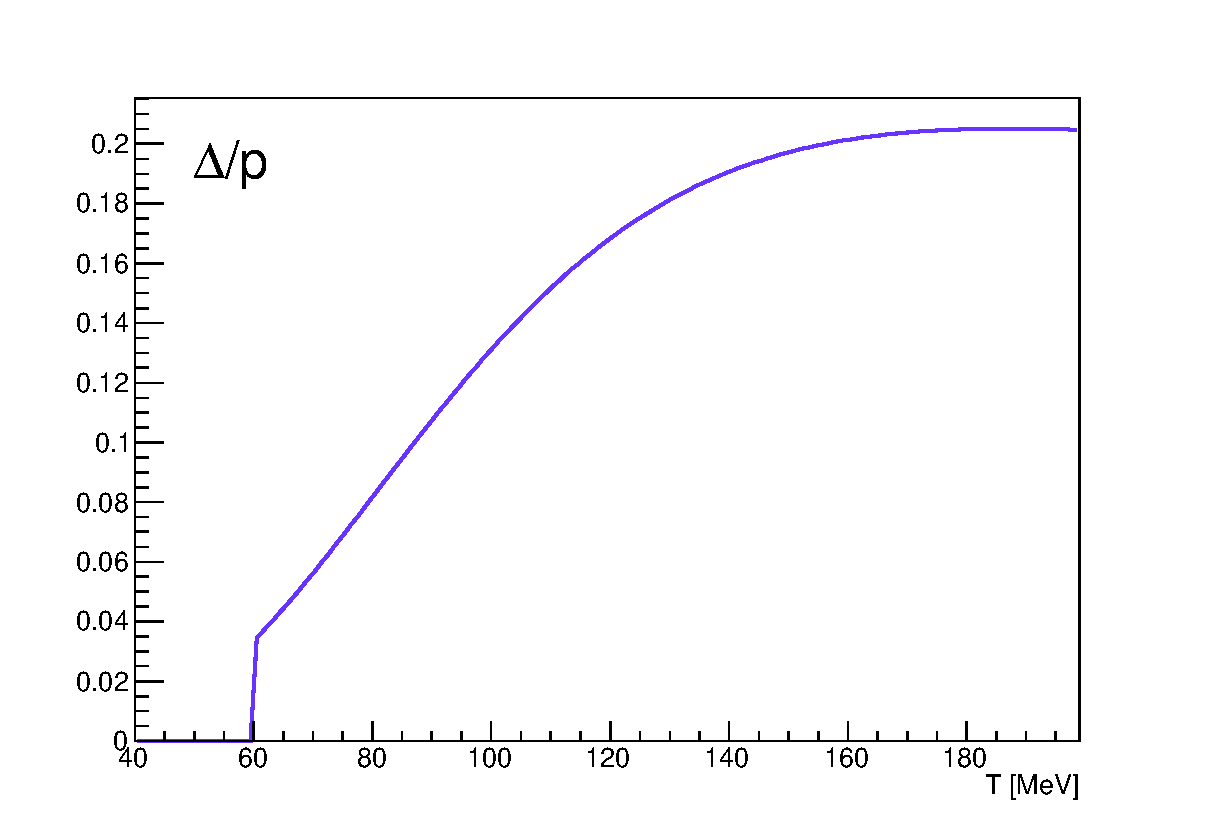
\includegraphics[width=200px]{./Version1/FigChapter2/DeltaToProton}
		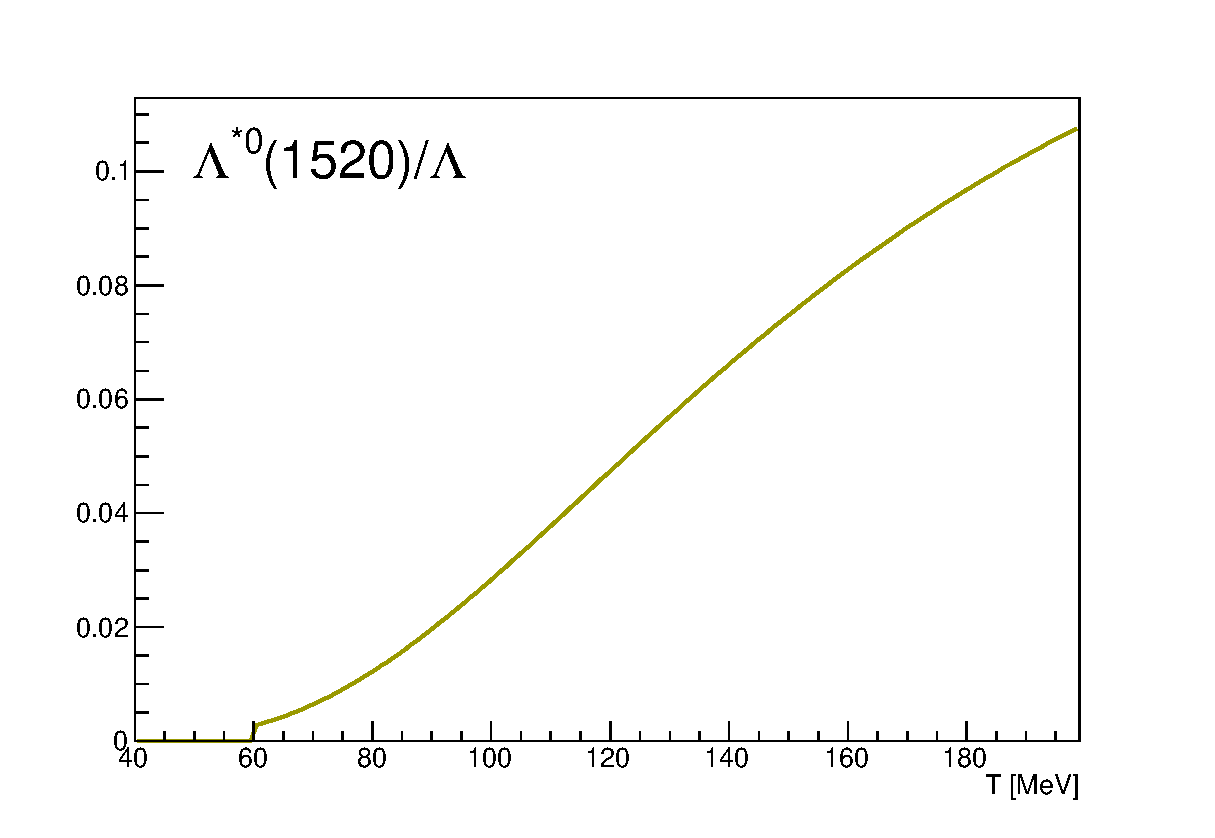
\includegraphics[width=200px]{./Version1/FigChapter2/LambdaStarToLambda}
		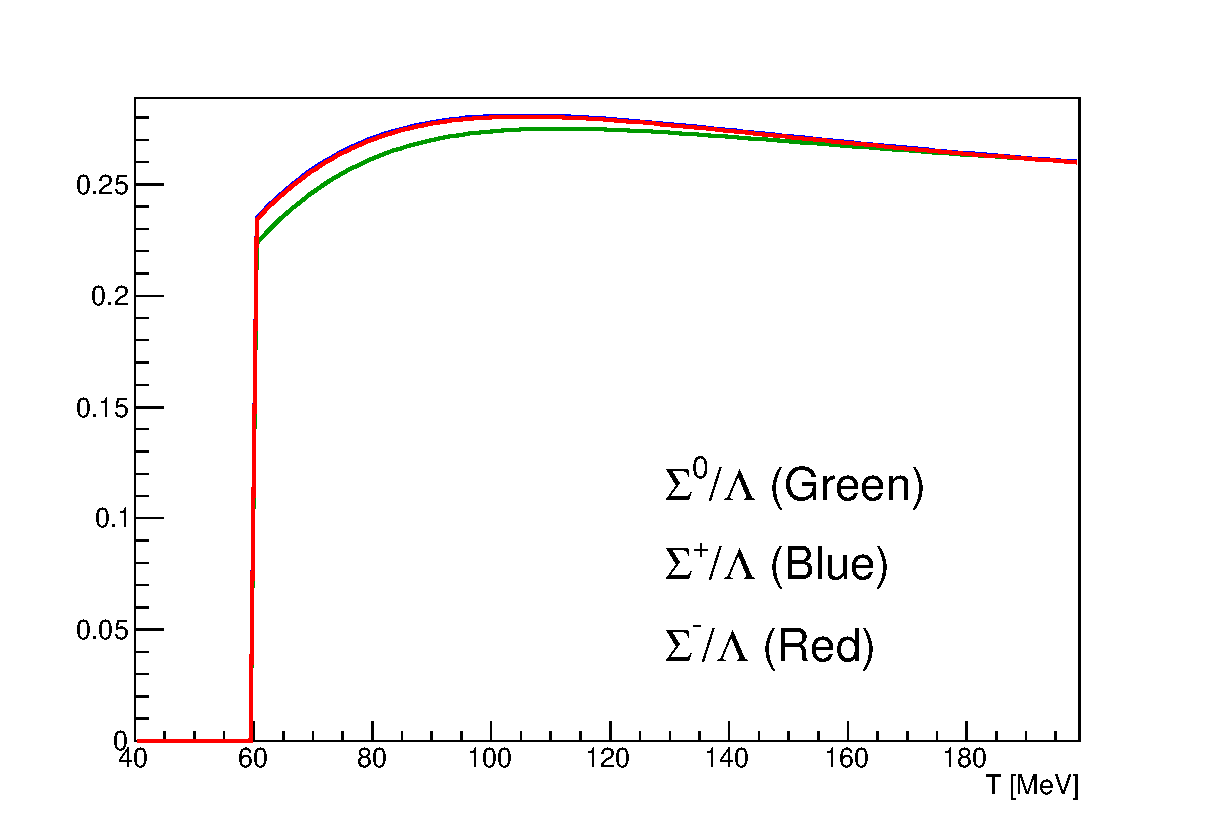
\includegraphics[width=200px]{./Version1/FigChapter2/SigmaRatio}
		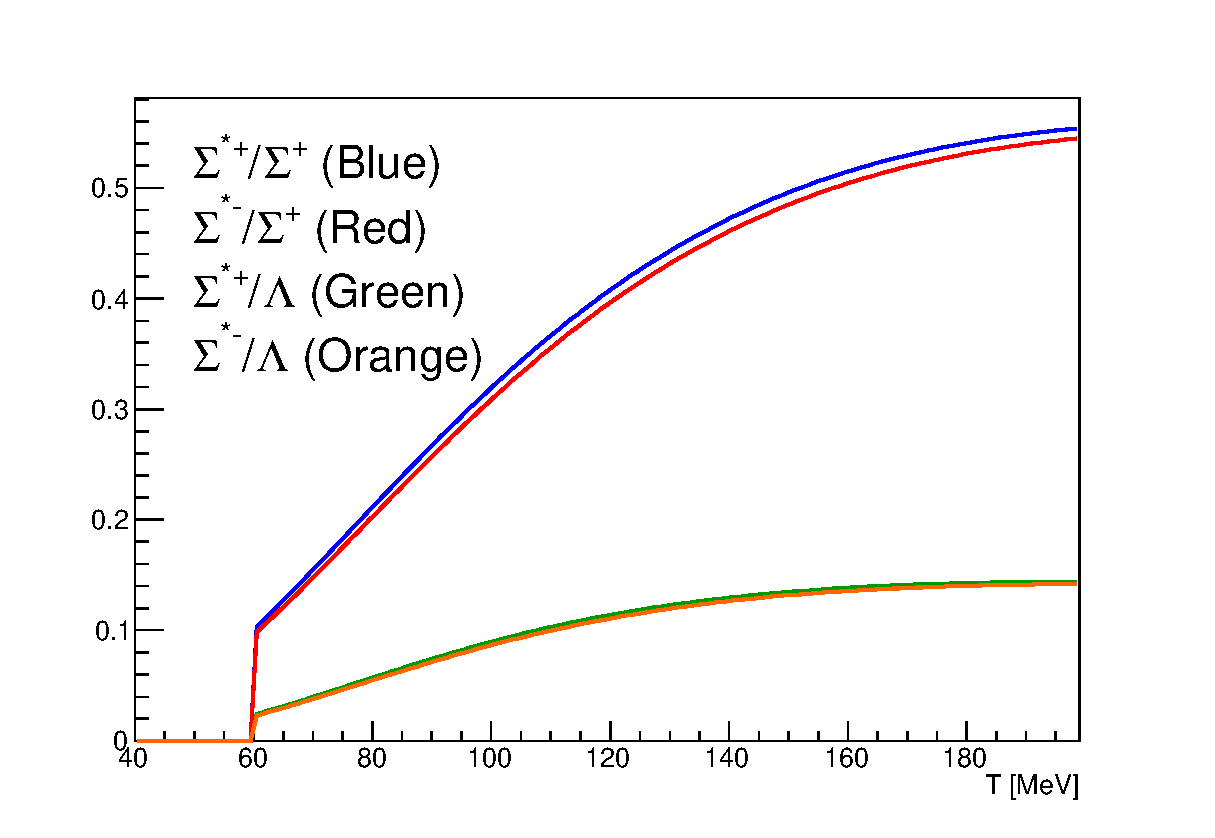
\includegraphics[width=200px]{./Version1/FigChapter2/SigmaStarRatio}
		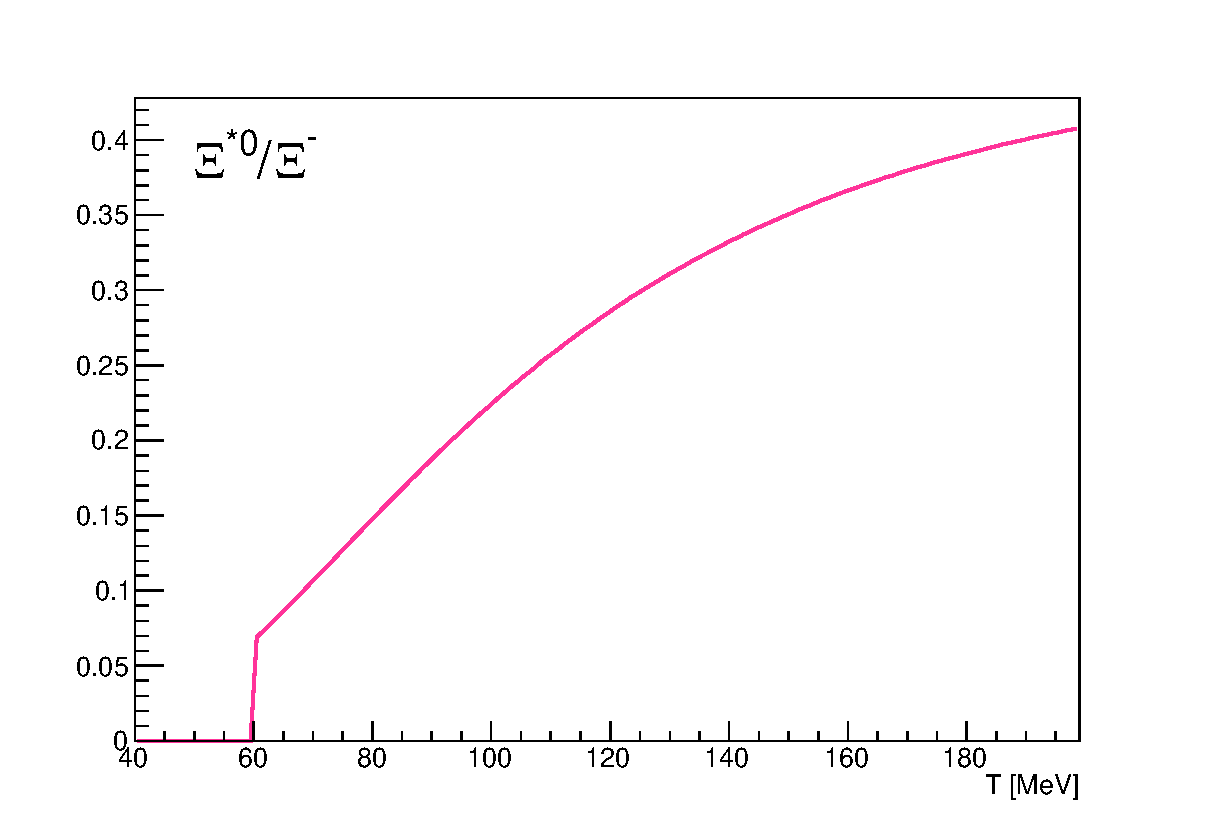
\includegraphics[width=200px]{./Version1/FigChapter2/XiStarToXi}
		\caption{\label{result1} Ratio of baryonic and mesonic resonances over their stable partner as a function of temperature.}
	\end{center}\hspace{2pc}%
\end{figure}




\begin{figure}[!htbp]
\begin{center}
	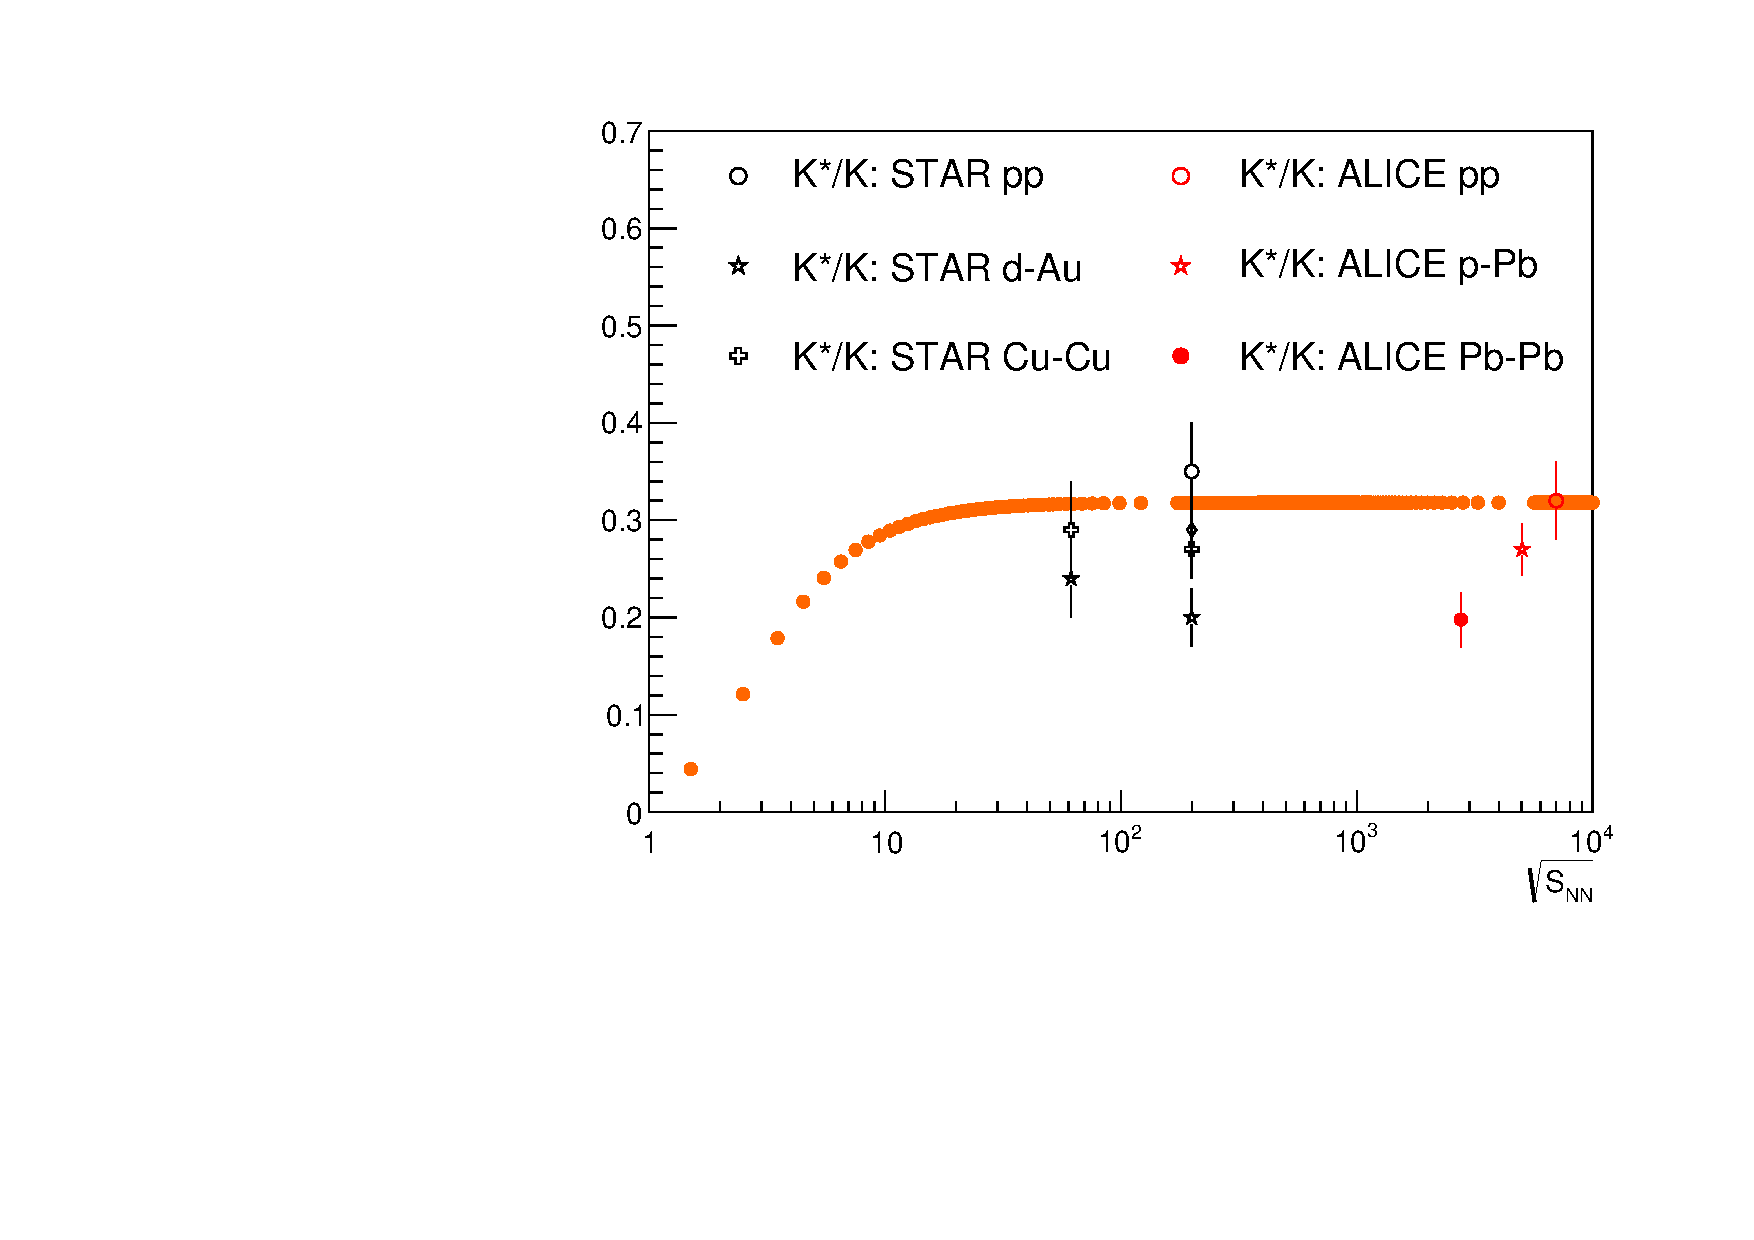
\includegraphics[width=200px]{./Version1/FigChapter2/Kstar_sqrt_s.pdf}
	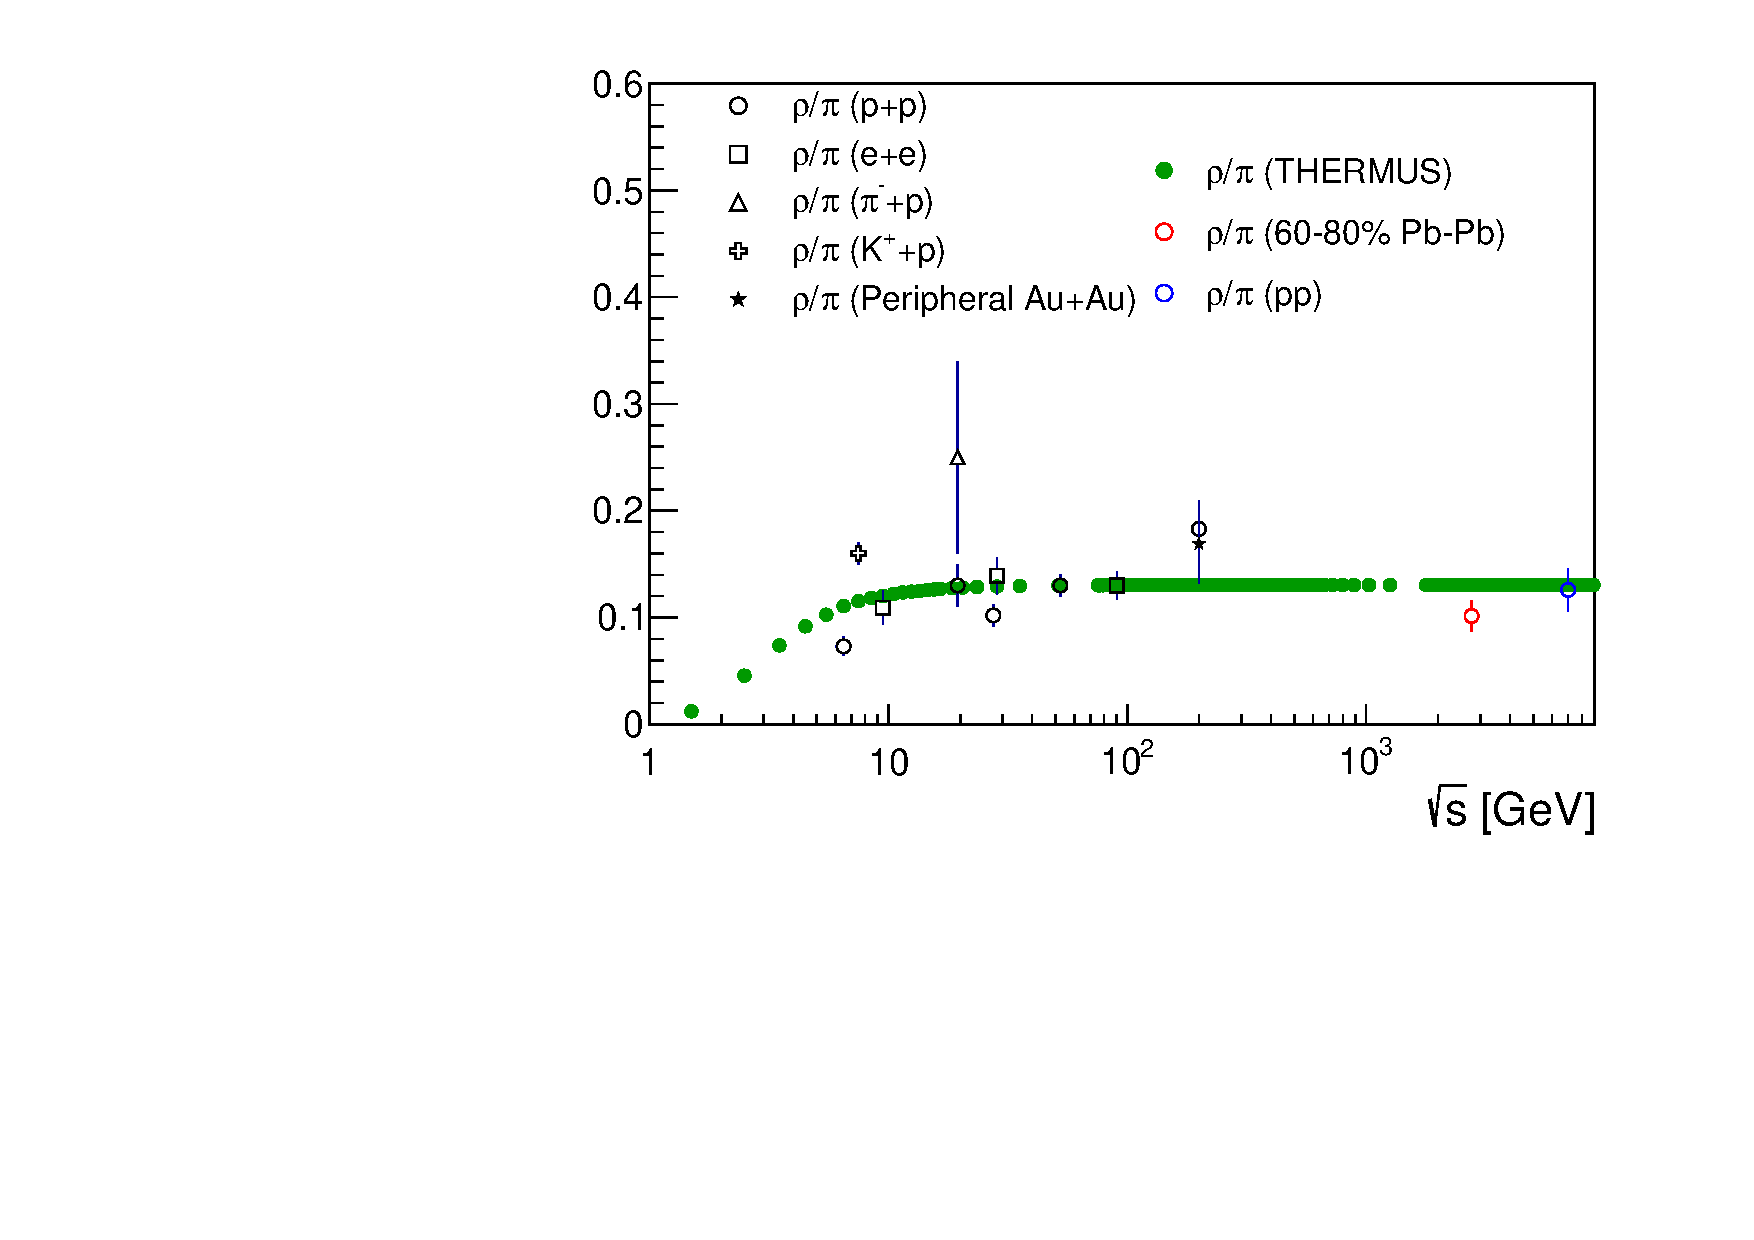
\includegraphics[width=200px]{./Version1/FigChapter2/RhoToPion_sqrt_s.pdf}
	\caption{\label{result2} Ratio of resonances over their stable partner as a function of $\sqrt{(s)}$.}
\end{center}\hspace{2pc}%
\end{figure}


\newpage

\subsection{EPOS, UrQMD}
The EPOS3 model \cite{cite:EPOSa, cite:EPOSb, cite:EPOSc} describes the full evolution of a heavy-ion collision. The initial stage is treated via a multiple-scattering approach based on Pomerons and strings. The reaction volume is divided into a core and a corona part \cite{cite:EPOSd}. The core is taken as the initial condition for the QGP evolution, for which one employ viscous hydrodynamics. The corona part is simply composed of hadrons from string decays. After hadronisation of the fluid (core part), these hadrons and as well the corona hadrons are fed into UrQMD \cite{cite:URQMDa, cite:URQMDb}, which describes hadronic interactions in a microscopic approach. The chemical and kinetic freeze-outs occur within this phase. The chemical freeze-out is expected to occur shortly after the phase transition from partonic to hadronic matter and is followed by the kinetic freeze-out.


As explained in \cite{cite:EPOSa, cite:EPOSb, cite:EPOSc, cite:EPOSd}, EPOS3 is an event generator based on 3+1D viscous hydrodynamical evolution starting from flux tube initial conditions, which are generated in the Gribov-Regge multiple scattering framework. An individual scattering is referred to as a Pomeron, identified with a parton ladder, eventually showing up as flux tubes (or strings). Each parton ladder is composed of a pQCD hard process, plus initial and final state linear parton emission. Nonlinear effects are considered by using saturation scales $Q_{s}$, depending on the energy and the number of participants connected to the Pomeron in question.


The final state partonic system (corresponding to a Pomeron) amounts to (usually two) color flux tubes, being mainly longitudinal, with transversely moving pieces carrying the \pt of the partons from hard scatterings. One has two flux tubes based on the cylindrical topology of the Pomerons. Each quark- antiquark pair in the parton ladder will cut a string into two; in this sense one may have more than two flux tubes. In any case, these flux tubes eventually constitute both bulk matter, also referred to as ?core? (which thermalizes, flows, and finally hadronizes) and jets (also referred to as ?corona?), according to some criteria based on the energy of the string segments and the local string density. For the core, we use a 3+1D viscous hydrodynamic approach, employing a realistic equation of state, compatible with lQCD results. We employ for all calculations in this paper a value of ?/s = 0.08. Whenever a hadronisation temperature of TH is reached, we apply the usual Cooper-Frye freeze-out procedure, to convert the fluid into particles. We use TH = 166MeV. From this point on, we apply the hadronic cascade UrQMD \cite{cite:URQMDa, cite:URQMDb}, about which more details are given later. All hadrons participate in the cascade, including those from the core (after freeze- out) and the corona. The corona particles, from string decay, are only ?visible? after a certain formation time (some constant of order one fm/c), multiplied by the corresponding gamma factor), so very high \pt particles have a good chance to escape.

The UrQMD model is a non-equilibrium transport approach. The interactions of hadrons in the current version include binary elastic and 2 $\rightarrow$ n inelastic scatterings, resonance creations and decays, string excitations, particle + antiparticle annihilations as well as strangeness exchange reactions. The cross sections and branching ratios for the corresponding interactions are taken from experimental measurements (where available), detailed balance relations and the additive quark model. The model describes the full phase-space evolution of all hadrons, including resonances, in a heavy- ion collision based on their hadronic interactions and their decay products. Due to the short lifetime of resonances, their decay products may interact in the hadronic phase. This is not the case for weak decays, where the system has already decoupled at the time of the decay. As discussed previously, the experimental reconstruction of resonances will be influenced by the final state interactions of the decay products. Resonance signals have been previously studied using the UrQMD model. 


\newpage